%  This is a LaTex file.

%  Homework for the course "AMath 585:  Applied Linear Algebra and Numerical Analysis", 
%  Autumn quarter, 2009, Anne Greenbaum.


%   A latex format for making homework assignments.


\documentclass[letterpaper,12pt]{article}

%          The page format, somewhat wider and taller page than in art12.sty.

\topmargin -0.1in \headsep 0in \textheight 8.9in \footskip 0.6in
\oddsidemargin 0in  \evensidemargin 0in  \textwidth 6.5in
\usepackage{graphicx}
\usepackage{listings}
\usepackage{caption}
\usepackage{subcaption}
\usepackage{color}
\usepackage{float}
\definecolor{keywords}{RGB}{255,0,90}
\definecolor{comments}{RGB}{0,0,113}
\definecolor{red}{RGB}{160,0,0}
\definecolor{green}{RGB}{0,150,0}
\definecolor{codegreen}{rgb}{0,0.6,0}
\definecolor{codegray}{rgb}{0.5,0.5,0.5}
\definecolor{codepurple}{rgb}{0.58,0,0.82}
\definecolor{backcolour}{rgb}{0.95,0.95,0.92}
\definecolor{brown}{rgb}{0.59, 0.29, 0.0}
\definecolor{beaublue}{rgb}{0.74, 0.83, 0.9}
\definecolor{orange}{rgb}{1.0, 0.5, 0.0}
\definecolor{darkslategray}{rgb}{0.18, 0.31, 0.31}
\definecolor{deepblue}{rgb}{0,0,0.5}
\definecolor{deepred}{rgb}{0.6,0,0}
\definecolor{deepgreen}{rgb}{0,0.5,0}
\lstdefinestyle{myMatlabstyle}{
	language=Matlab,
	backgroundcolor=\color{white},   
	commentstyle=\color{codegreen},
	keywordstyle=\color{blue},
	identifierstyle=\color{brown},
	numberstyle=\tiny\color{codegray},
	stringstyle=\color{orange},
	basicstyle=\footnotesize,
	breakatwhitespace=false,         
	breaklines=true,                 
	captionpos=b,                    
	keepspaces=true,                 
	numbers=left,                    
	numbersep=5pt,                  
	showspaces=false,                
	showstringspaces=false,
	showtabs=false,                  
	tabsize=2
}
\lstdefinestyle{myPythonstyle}{
	language=Python, 
	basicstyle=\ttfamily\small, 
	keywordstyle=\color{blue},
	commentstyle=\color{green},
	stringstyle=\color{red},
	showstringspaces=false,
	identifierstyle=\color{black},
}
\lstset{language=Matlab,frame=single}
\lstset{language=Python,frame=single}
\usepackage{amsmath}
\usepackage{amsmath,amsfonts,amsthm} % 
\usepackage{epsfig}         % to insert PostScript figures

\begin{document}


%          Definitions of commonly used symbols.



%          The title and header.

\noindent
{\scriptsize AMath 585, Winter 2018} \hfill 

\begin{center}
\large
Assignment 2. 
\normalsize

Jithin D. George, No. 1622555

\end{center}
\noindent
Due Monday, Jan. 22.
\vspace{.3in}




\begin{enumerate}
\item (Inverse matrix and Green's functions)
\begin{enumerate}
\item Write out the $5\times 5$
matrix $A$ from (2.43) for the boundary value problem
$u''(x)=f(x)$ with $u(0)=u(1)=0$ for  $h = 0.25$.


{\bf Solution:}


\[A = \begin{bmatrix}
        1. & 0. & 0. & 0. & 0.\\
        0.25 & -0.5 & 0.25 & 0. & 0.\\ 
        0. & 0.25 & -0.5 & 0.25 & 0.\\ 
        0. & 0. & 0.25 & -0.5 & 0.25\\ 
        0. & 0. & 0. & 0. & 1.\\
        \end{bmatrix} \]


\item Write out the $5\times 5$
inverse matrix $A^{-1}$ explicitly for this problem.

{\bf Solution:}


 \[A^{-1} =\begin{bmatrix} 1. & -0. & -0. & -0. & 0.\\ 0.75 & -0.046875 & -0.03125 & -0.015625 & 0.25\\  0.5 & -0.03125 & -0.0625 & -0.03125 & 0.5\\  0.25 & -0.015625 & -0.03125 & -0.046875 & 0.75\\  0. & 0. & 0. & 0. & 1. \end{bmatrix}\]

\item
If $f(x)=x$, determine the discrete approximation to the solution of the
boundary value problem on this grid and sketch this solution and the five
Green's functions whose sum gives this solution.

{\bf Solution:}

\[u(x) = \int_0^1 \bar{x}  G(x; \bar{x} )\,d \bar{x} =  0.25h G_1 + 0.5h G_2 + 0.75h G_3 \]

\begin{figure}[H]

\centering
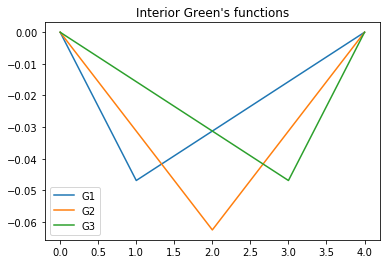
\includegraphics[width=.3\textwidth]{int.png}\hfill
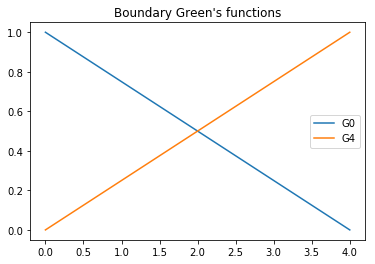
\includegraphics[width=.3\textwidth]{bound.png}\hfill
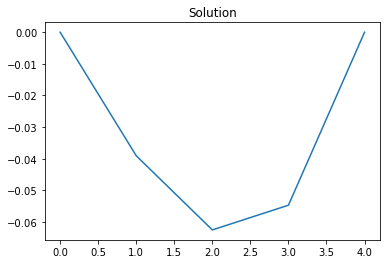
\includegraphics[width=.3\textwidth]{solution.png}

\caption{Interior Green's functions, Boundary Green's functions and Solution}
\label{fig:figure3}

\end{figure}


\end{enumerate}

\item (Another way of analyzing the error using Green's functions)
The {\em composite trapezoid rule} for integration approximates the
integral from $a$ to $b$ of a function $g$ by dividing the interval
into segments of length $h$ and approximating the integral over each
segment by the integral of the linear function that matches $g$ at
the endpoints of the segment. (For $g > 0$, this is the area of
the trapezoid with height $g( x_j )$ at the left endpoint $x_j$
and height $g( x_{j+1} )$ at the right endpoint $x_{j+1}$.)  Letting
$h = (b-a)/(m+1)$ and $x_j = a + jh$, $j = 0,1, \ldots , m, m+1$:
\[
\int_a^b g(x)\,dx \approx  h \sum_{j=0}^m \frac{g( x_j )+g( x_{j+1} )}{2} 
     =  h \left[ \frac{g( x_0 )}{2} + \sum_{j=1}^m g( x_j ) + 
                   \frac{g( x_{m+1} )}{2} \right] .
\]

\begin{enumerate}
\item
Assuming that $g$ is sufficiently smooth, show that the error in the 
composite trapezoid rule approximation to the integral is $O( h^2 )$.
[Hint:  Show that the error on each subinterval is $O( h^3 )$.]


{\bf Solution:}

\[g(x) = g(x_i) +g'(x_i)(x-x_i) +\frac{1}{2}g''(x_i)(x-x_i)^2 +O((x-x_i)^3) \]
\[\int_{x_i}^{x_{i+1}} g(x)dx = \int_{x_i}^{x_{i+1}} g(x_i)dx + \int_{x_i}^{x_{i+1}} g'(x_i)(x-x_i)dx + O((x_{i+1}-x_i)^3) dx \]
\[= g(x_i)(x_{i+1}-x_i) + g'(x_i)(x_{i+1}-x_i)^2 + O((x_{i+1}-x_i)^3)  \]
\begin{equation}
\int_{x_i}^{x_{i+1}} g(x)dx = g(x_i)h + g'(x_i)\frac{h^2}{2} + O(h^3)  
\end{equation}

\[g(x) = g(x_{i+1}) +g'(x_{i+1})(x-x_{i+1}) +\frac{1}{2}g''(x_{i+1})(x-x_{i+1})^2 +O((x-x_i)^3) \]
\[g(x) = g(x_{i+1}) +g'(x_{i})(x-x_{i+1}) +g''(x_{i})h(x-x_{i+1}) +\frac{1}{2}g''(x_{i+1})(x-x_{i+1})^2 +O((x-x_i)^3) \]
\[\int_{x_i}^{x_{i+1}}g(x)dx = \int_{x_i}^{x_{i}}g(x_{i+1})dx +\int_{x_i}^{x_{i+1}} g'(x_{i+1})(x-x_{i+1}) +O((x_{i+1}-x_i)^3) \]
\begin{equation}
\int_{x_i}^{x_{i+1}} g(x)dx = g(x_{i+1})h - g'(x_i)\frac{h^2}{2} + O(h^3)  
\end{equation}
Adding (1) and (2) together,
\[\int_{x_i}^{x_{i+1}} g(x)dx = \frac{h}{2}(g(x_{i})+g(x_{i+1})) + O(h^3) \]
\item
Recall that the true solution of the boundary value problem $u'' (x) = f(x)$,
$u(0) = u(1) = 0$ can be written as
\begin{equation}
u(x) = \int_0^1 f( \bar{x} ) G(x; \bar{x} )\,d \bar{x} , \label{1}
\end{equation}
where $G(x; \bar{x})$ is the Green's function corresponding to
$\bar{x}$.  The finite difference approximation $u_i$ to $u( x_i )$, 
using the centered finite difference scheme in (2.43), is
\begin{equation}
u_i = h \sum_{j=1}^m f( x_j ) G( x_i ; x_j ) ,~~i=1, \ldots , m . \label{2}
\end{equation}
Show that formula (\ref{2}) is the trapezoid rule approximation to 
the integral in (\ref{1}) when $x = x_i$, and conclude from this that the 
error in the finite difference approximation is $O( h^2 )$ at each node $x_i$. 
[Recall:  The Green's function $G( x ; x_j )$ has a {\em discontinuous}
derivative at $x = x_j$.  Why does this not degrade the accuracy of the
composite trapezoid rule?]


{\bf Solution:}

\[u(x) = \int_0^1 f( \bar{x} ) G(x; \bar{x} )\,d \bar{x}\]
Setting x = $x_i$ and using the Trapezoidal approximation,
\[u_i =   h \frac{ f( 0 ) G( x_i ; 0 )}{2} + h \sum_{j=1}^m f( x_j ) G( x_i ; x_j )+  h \frac{ f( 1 ) G( x_i ; 1 )}{2} \]
Since the Green's function is the solution to the ODE and since at the boundaries, u is 0, G(x,0)=G(x,1)=0.
So, we get
\[u_i = h \sum_{j=1}^m f( x_j ) G( x_i ; x_j )\]
\end{enumerate}

\item (Green's function with Neumann boundary conditions)
\begin{enumerate}
\item
Determine the Green's functions for the two-point boundary
value problem $u''(x) = f(x)$ on $0<x<1$ with a Neumann boundary condition
at $x=0$ and a Dirichlet condition at $x=1$, i.e, find the function
$G(x,\bar x)$ solving
\[
u''(x) = \delta(x-\bar x), \quad u'(0)=0, \quad u(1)=0
\]
and the functions $G_0(x)$ solving
\[
u''(x) = 0, \quad u'(0)=1, \quad u(1)=0
\]
and $G_1(x)$ solving
\[
u''(x) = 0, \quad u'(0)=0, \quad u(1)=1.
\]


{\bf Solution:}

 We need 
 \[u'(0)=0 , u(1)=0 \]
 and
 \[u(\bar{x}+\epsilon)-u(\bar{x}-\epsilon)=1\]
 So, the Green's function satisying that would be given by

  \[
    G(x,\bar{x}) = \left\{\begin{array}{lr}
        \bar{x}-1, & \text{for } 0\leq x\leq \bar{x}\\

        x-1, & \text{for } \bar{x}\leq x\leq 1
        \end{array}\right\} \]

Solving the odes for the boundaries, we have
\[G_0(x) = x-1\]
\[G_1(x) = 1\]
\item
Using this as guidance, find the general formulas for the elements of the
inverse of the matrix in equation (2.54).  Write out the $5\times 5$ matrices
$A$ and $A^{-1}$ for the case $h=0.25$.

{\bf Solution:}


\[A = \begin{bmatrix}
        3. & -4. & 1. & 0. & 0.\\
        0.25 & -0.5 & 0.25 & 0. & 0.\\ 
        0. & 0.25 & -0.5 & 0.25 & 0.\\ 
        0. & 0. & 0.25 & -0.5 & 0.25\\ 
        0. & 0. & 0. & 0. & 1.\\
        \end{bmatrix} \]
        
\[A^{-1} = 
\begin{bmatrix}  -1. & -0.75 & -0.5 & -0.25 & 1.\\  -0.75 & -0.75 & -0.5 & -0.25 & 1.\\  -0.5 & -0.5 & -0.5 & -0.25 & 1.\\  -0.25 & -0.25 & -0.25 & -0.25 & 1.\\ 0. & 0. & 0. & 0. & 1.  \end{bmatrix}
\]

\end{enumerate}


\item (Solvability condition for Neumann problem)
Determine the null space of the matrix $A^T$, where $A$ is given in
equation (2.58), and verify that the condition (2.62) must hold for the
linear system to have solutions.

{\bf Solution:}


\[
A= \left( \begin{array}{cccccc}
-h & h &        &        &    &  \\
1  & -2 & 1      &        &    &  \\
   & 1  & \ddots & \ddots &     & \\
   &    & \ddots & \ddots & 1    & \\
   &    &        & 1      & -2 & 1 \\
      &    &        &       & h & -h \\
   \end{array} \right)
\]
\[
A^T= \left( \begin{array}{cccccc}
-h & 1 &        &        &    &  \\
h  & -2 & 1      &        &    &  \\
   & 1  & \ddots & \ddots &     & \\
   &    & \ddots & \ddots & 1    & \\
   &    &        & 1      & -2 & h \\
      &    &        &       & 1 & -h \\
   \end{array} \right)
\]
The nullspace of this matrix is the vector [1,h,h,h,h....,h,1] because we can see multiplying them yields 0.
So, a solution only exists if the f-vector is orthogonal to the nullspace. Setting the dot-product equal to 0, we obtain the following criteria
\[ \sigma_0 + (h/2) f( x_0 )  +  h f( x_1 ) +\hdots + 
h f( x_{m-1} ) +  h f( x_m ) - \sigma_1  +  \frac{h}{2} f( x_{m+1} ) = 0 \]
which is the same as 2.62.
\item (Symmetric tridiagonal matrices)
\begin{enumerate}
\item
Consider the {\bf Second approach} described on p.~31 for dealing with
a Neumann boundary condition.  If we use this technique to approximate
the solution to the boundary value problem $u'' (x) = f(x)$, 
$0 \leq x \leq 1$, $u' (0) = \sigma$, $u(1) = \beta$, then the resulting
linear system $A {\bf u} = {\bf f}$ has the following form:
\[
\frac{1}{h^2} \left( \begin{array}{ccccc}
-h & h  &        &        &      \\
1  & -2 & 1      &        &      \\
   & 1  & \ddots & \ddots &      \\
   &    & \ddots & \ddots & 1    \\
   &    &        & 1      & -2 \end{array} \right)
\left( \begin{array}{c} u_0 \\ u_1 \\ \vdots \\ u_{m-1} \\ u_{m} \end{array} 
\right) =
\left( \begin{array}{c} \sigma + (h/2) f( x_0 ) \\ f( x_1 ) \\ \vdots \\ 
f( x_{m-1} ) \\ f( x_m ) - \beta / h^2 \end{array} \right) .
\]
Show that the above matrix is similar to a symmetric tridiagonal matrix 
via a {\em diagonal} similarity transformation; that is, there is a diagonal
matrix $D$ such that $D A D^{-1}$ is symmetric.

{\bf Solution:}
Experimenting with a smaller version,
\[
\left( \begin{array}{ccccc}
d_0 &   &     0       \\
0  & d_1 & 0        \\

0       & 0      & d_2 \end{array} \right) \left( \begin{array}{ccccc}
-h & h  &     0       \\
1  & -2 & 1        \\

0       & 1      & -2 \end{array} \right) 
\left( \begin{array}{ccccc}
\frac{1}{d_0} &   &     0       \\
0  & \frac{1}{d_1} & 0        \\

0       & 0      & \frac{1}{d_2} \end{array} \right) =
 \left( \begin{array}{ccccc}
-h & h\frac{d_0}{d_1}  &     0       \\
\frac{d_1}{d_0}  & -2 & \frac{d_1}{d_2}       \\

0       & \frac{d_2}{d_1}      & -2 \end{array} \right)\]

So, for the resulting matrix to be symmetric, we choose
the diagonal vector given by [1 $\sqrt{h}$ $\sqrt{h}$ $\sqrt{h}$  $\sqrt{h}$]

\[
\left( \begin{array}{ccccc}
1 &   &        &        &      \\
  & \sqrt{h} &      &        &      \\
   &   & \ddots & &      \\
   &    &  & \ddots &    \\
   &    &        &       & \sqrt{h} \end{array} \right) \left( \begin{array}{ccccc}
-h & h  &        &        &      \\
1  & -2 & 1      &        &      \\
   & 1  & \ddots & \ddots &      \\
   &    & \ddots & \ddots & 1    \\
   &    &        & 1      & -2 \end{array} \right)
   \left( \begin{array}{ccccc}
1 &   &        &        &      \\
  & \frac{1}{\sqrt{h}} &      &        &      \\
   &   & \ddots & &      \\
   &    &  & \ddots &    \\
   &    &        &       & \frac{1}{\sqrt{h}} \end{array} \right) \]
   
  \[ =  \left( \begin{array}{ccccc}
-h & \sqrt{h} &        &        &      \\
\sqrt{h}  & -2 & 1      &        &      \\
   & 1  & \ddots & \ddots &      \\
   &    & \ddots & \ddots & 1    \\
   &    &        & 1      & -2 \end{array} \right)\]
   This is a symmetric matrix.
\item
Consider the {\bf Third approach} described on pp.~31-32 for dealing with
a Neumann boundary condition.  [{\bf Note:} If you have an older edition of the text,
there is a typo in the matrix (2.57) on p.~32.  There should be a row above what is written
there that has entries $\frac{3}{2} h$, $-2h$, and $\frac{1}{2} h$
in columns $1$ through $3$ and $0$'s elsewhere.  I believe this was corrected in newer editions.]  
Show that if we use that first equation
(given at the bottom of p. 31) to eliminate $u_0$ and we also eliminate
$u_{m+1}$ from the equations by setting it equal to $\beta$ and modifying
the right-hand side vector accordingly, then we obtain an $m$ by $m$
linear system $A {\bf u} = {\bf f}$, where $A$ is similar to a symmetric
tridiagonal matrix via a diagonal similarity transformation.

{\bf Solution:}

\[
\frac{1}{h^2} \left( \begin{array}{ccccc}
\frac{3}{2}h & -2h  & \frac{1}{2}h       &        &      \\
1  & -2 & 1      &        &      \\
   & 1  & \ddots & \ddots &      \\
   &    & \ddots & \ddots & 1    \\
   &    &        & 1      & -2 \end{array} \right)
\left( \begin{array}{c} u_0 \\ u_1 \\ \vdots \\ u_{m-1} \\ u_{m} \end{array} 
\right) =
\left( \begin{array}{c} \sigma  \\ f( x_1 ) \\ \vdots \\ 
f( x_{m-1} ) \\ f( x_m ) - \beta / h^2 \end{array} \right) .
\]
\[
\frac{1}{h^2} \left( \begin{array}{ccccc}
3 & -4  & 1       &        &      \\
3  & -6 & 3      &        &      \\
   & 1  & \ddots & \ddots &      \\
   &    & \ddots & \ddots & 1    \\
   &    &        & 1      & -2 \end{array} \right)
\left( \begin{array}{c} u_0 \\ u_1 \\ \vdots \\ u_{m-1} \\ u_{m} \end{array} 
\right) =
\left( \begin{array}{c} 2 \frac{\sigma}{h}  \\ 3f( x_1 ) \\ \vdots \\ 
f( x_{m-1} ) \\ f( x_m ) - \beta / h^2 \end{array} \right) .
\]
Eliminating the boundary element,
\[
\frac{1}{h^2} \left( \begin{array}{ccccc}
 -1 & 1      &        &      \\
1  & \ddots & \ddots &      \\
    & \ddots & \ddots & 1    \\
   &        & 1      & -2 \end{array} \right)
\left( \begin{array}{c}  u_1 \\ \vdots \\ u_{m-1} \\ u_{m} \end{array} 
\right) =
\left( \begin{array}{c}  \frac{3}{2} f( x_1 ) -  \frac{\sigma}{h}  \\ \vdots \\ 
f( x_{m-1} ) \\ f( x_m ) - \beta / h^2 \end{array} \right) .
\]
   This is a symmetric matrix.
\end{enumerate}

\end{enumerate}

\end{document}
